% xetex compatible variant that support TTF fonts according to company rules
\documentclass[ignorenonframetext, professionalfonts, hyperref={unicode}]{beamer}

\usetheme{Epam}

\usepackage{fontspec}
\setsansfont{SourceSansPro-Regular}
%\setbeamerfont{frametitle}{family=\fontspec{Oswald}}
\setbeamerfont{frametitle}{family=\fontspec{Oswald}}
\setbeamerfont{block title}{family=\fontspec{Oswald}}

%\setmainfont{Times New Roman}
\defaultfontfeatures{Mapping=tex-text}
\defaultfontfeatures{Ligatures=TeX}

%\setsansfont{Arial}
%\setromanfont{Trebuchet MS}

\usepackage{cmap}
\usepackage{graphicx}

\usepackage{textcomp}

\usepackage{beamerthemesplit}

\usepackage{ulem}

\usepackage{verbatim}
\usepackage{import}

\usepackage{listings}
\lstloadlanguages{bash}

\lstset{escapechar=`,
	captionpos=b,
	extendedchars=false,
	language=sh,
%	frame=single,
	tabsize=2, 
	columns=fullflexible, 
%	basicstyle=\scriptsize,
	keywordstyle=\color{blue}, 
	commentstyle=\itshape\color{brown},
%	identifierstyle=\ttfamily, 
	stringstyle=\mdseries\color{green}, 
	showstringspaces=false, 
	numbers=left, 
	numberstyle=\footnotesize, 
	breaklines=true, 
	inputencoding=utf8,
	keepspaces=true,
	morekeywords={u\_short, u\_char, u\_long, in\_addr}
	}

\definecolor{darkgreen}{cmyk}{0.7, 0, 1, 0.5}

\lstdefinelanguage{diff}
{
    morekeywords={+, -},
    sensitive=false,
    morecomment=[l]{//},
    morecomment=[s]{/*}{*/},
    morecomment=[l][\color{darkgreen}]{+},
    morecomment=[l][\color{red}]{-},
    morestring=[b]",
}

\author[Epam]{{\bf Epam}\\Low Level Programming Department}

%\institution[EPAM]{EPAM}
%\logo{\includegraphics[width=1cm]{logo.png}}

\graphicspath{{../../slides/cmdline/clipart/}{../../slides/bash/clipart/}}

\bibliographystyle{unsrt}
\setbeamertemplate{bibliography item}{\insertbiblabel}

\AtBeginSection[]{%
  \begin{frame}<beamer>
    \frametitle{}
    \tableofcontents[
        sectionstyle=show/shaded, hideallsubsections ]
  \end{frame}
  \addtocounter{framenumber}{-1}% If you don't want them to affect the slide number
}

% \regex for regular expressions
\newcommand{\regex}[1]{ %
\expandafter{$\ulcorner{\color{blue}\texttt{#1}}\lrcorner$} %
}



\title{Введение в GNU/Linux}

%%%%%%%%%%%%%%%%%%%%%%%%%%%%%%%%%%%%%%%%%%%%%%%%%
%%%%%%%%%% Begin Document  %%%%%%%%%%%%%%%%%%%%%%
%%%%%%%%%%%%%%%%%%%%%%%%%%%%%%%%%%%%%%%%%%%%%%%%%

\begin{document}

\begin{frame}
	\frametitle{Web application.}
	\titlepage
	\vspace{-0.5cm}
	\begin{center}
	%\frontpagelogo
	\end{center}
\end{frame}


\begin{frame}
	\tableofcontents
	[hideallsubsections]
\end{frame}

%%%%%%%%%%%%%%%%%%%%%%%%%%%%%%%%%%%%%%%%%   
%%%%%%%%%% Content starts here %%%%%%%%%%
%%%%%%%%%%%%%%%%%%%%%%%%%%%%%%%%%%%%%%%%%

\section{Database}
\mode<all>{\begin{frame}[fragile]
        \frametitle{Database client server}
    
    \alert{Server} - the database server program
\begin{itemize}
    \item manages the database files;
    \item accepts connections to the database from client applications;
    \item performs database actions on behalf of the clients.
\end{itemize}
\alert{Client} - application that wants to perform database operations
\begin{itemize}
    \item text-oriented tool
    \item a graphical application,
    \item a web server that accesses the database to display web pages,
    \item a specialized database maintenance tool
\end{itemize}

\end{frame}
}
\mode<all>{\begin{frame}[fragile]
        \frametitle{Database example}
Database is collection of tables
\begin{itemize}
    \item Table contains rows and columns
    \item Tables may have relationships
\end{itemize}

Activities Table
\begin{tabular}{| c | c | c | c | c |}
   \hline
   Student     & Activity1 & Cost1 & Activity2 & Cost2 \\ 
   \hline 
   John Smith  & Tennis    & \$36  & Swimming  & \$17  \\
   Jane Bloggs & Squash    & \$40  & Swimming  & \$17  \\
   John Smith  & Tennis    & \$36  &           &       \\
   Mark Antony & Swimming  & \$15  & Golf      & \$47  \\ 
   \hline
\end{tabular}

\end{frame}

\begin{frame}[fragile]
        \frametitle{Database example}
        \center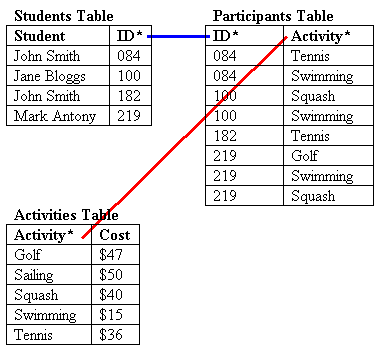
\includegraphics[width=0.7\textwidth]{../../slides/web/media/db_table.png}
\end{frame}
}
\section{SQL}
\mode<all>{\begin{frame}[fragile]
        \frametitle{Structured query language SQL}

\begin{itemize}
   \item Data definition (Schema)
   \item Data manipulation
\end{itemize}


Database Schema example
\begin{lstlisting}[language=sql]
CREATE TABLE music ( Title TEXT, Author TEXT);
\end{lstlisting}

Data manipulation example
\begin{lstlisting}[language=sql]
INSERT INTO music VALUES ('My Life','Dr Alban');
DROP TABLE music;
\end{lstlisting}

\end{frame}
}
\mode<all>{\begin{frame}[fragile]
        \frametitle{SQL common operations}

\begin{itemize}
\item INSERT
\item UPDATE
\item DELETE
\item SELECT * FROM table;
\item SELECT COUNT()
\end{itemize}
CRUD - create read update delete

\end{frame}
}
\mode<all>{\begin{frame}[fragile]
        \frametitle{SQL Select example}

Data manipulation example
\begin{lstlisting}[language=sql]
SELECT *
FROM sites
WHERE site_name = 'TechOnTheNet.com'
ORDER BY site_id ASC;
\end{lstlisting}

\end{frame}
}
\section{MySQL. MariaDB.}
\mode<all>{\begin{frame}[fragile]
        \frametitle{Implementations}

\begin{itemize}
   \item MariaDB (former MySQL)
   \item PostgresSQL
   \item Oracle
\end{itemize}

SQL vendor specific syntax and functions

\end{frame}
}
\section{Access management.}
\mode<all>{\begin{frame}[fragile]
        \frametitle{MariaDB add privileges}

\begin{lstlisting}[language=sql]
GRANT ALL PRIVILEGES ON *.* TO
'yourusername'@'localhost' IDENTIFIED BY
'yourpassword' WITH GRANT OPTION;
\end{lstlisting}

\begin{lstlisting}[language=sql]
GRANT SELECT, INSERT, UPDATE, DELETE, CREATE, DROP, INDEX, ALTER, CREATE
TEMPORARY TABLES, LOCK TABLES ON
database1.* TO 'yourusername'@'localhost'
IDENTIFIED BY 'yourpassword';
\end{lstlisting}

\end{frame}
}

\end{document}
